\documentclass[12pt]{article} \usepackage[margin=1in]{geometry}

\usepackage{graphicx}
\usepackage{color}

%% \usepackage{amsmath}
%% \usepackage{listings}

%% \lstloadlanguages{C++} \lstset{ language=C++, breaklines=true,
%%   keywordstyle=\color{blue}, commentstyle=\color{red} }


\newenvironment{listing}%
               {\begin{table}
                   \begin{tabular}{ p{6in} }
                     \hline}%
               {\end{tabular}%
               \end{table}}


\begin{document}

\title{A New Algorithm for Second Order Perturbation Theory}
\author{Andrey Asadchev \and Mark S. Gordon}
\date{}

\maketitle


\abstract{
A new second order perturbation theory (MP2) algorithm is presented
for closed shell energy evaluations. The new algorithm has a
significantly lower memory footprint, a lower FLOP (floating point
operations) count, and a transparent approach for the disk/distributed
memory storage of the MP2 amplitudes. The algorithm works equally well
on single workstations and large clusters. The new algorithm allows
one to perform large calculations with thousands of basis functions in
a matter of hours on a single workstation. While for most practical
purposes, classical MP2 is eclipsed by density-fitting methods, the
approaches and lessons learned in the presented implementation are
applicable beyond the MP2 algorithm.
}


\section{Introduction}
The integral transformation, also known as 4-index tranformation,
tranforms atomic (typically) integrals to molecular integrals via the
simple formula:

$$(ij|kl) = C(i,p)C(j,q)C(k,r)C(l,s)(pq|rs)$$

Using the common convention, occupied indices $o$ are designated by
indices $i,j,...$, virtual indices $v$ are designated by indices $a,
b,...$, and atomic indices $n$ by indices $p,q,r,s$.

Typically, several classes of molecular integrals are needed, eg
$(ai|bj)$, $(ab|ci)$, etc.  But in the case of MP2 energy,

$$t_{ij}^{ab} = \frac{2 (ai|bj) - (bi|aj)}{\epsilon_i + \epsilon_j - \epsilon_a -
  \epsilon_b}$$
$$E_{MP2} = \sum \sum t_{ij}^{ab}(ai|bj)$$

only $(ai|bj)$ integrals are needed to form $t_{ij}^{ab}$ MP2
amplitudes.  The $(ai|bj)$ integrals and consequently $t$ amplitude
have symmetry such that $(ai|bj) = (bj|ai)$ which can be used to halve
storage requirement and number of computations.

The MP2 energy calculation scales as $O N^4$ and requires $O^2 V^2$
integral storage. Out of all many body methods is the cheapest and the
one with lowest compute to I/O ratio.

There is a number of different algorithms developed over the years,
\cite{head1988MP2, frisch1990semi, wong1996parallel,schutz1997integral,
  fletcher1997parallel, ford2007array, ishimura2006new}
due to simplicity of the algorithm and its popularity.
This work is to improve the algorithm and generalize it to handle
larger calculations, using either memory or filesystem as a storage
medium.

\section {Matrix chaining}
There exists a simple matrix chaining multiplication property, which,
surprisingly, is not very well-known.  Given three (or more) matrices,
the matrices can be multiplied without changing the outcome by two
different factorizations, $A = (BC)D$ and $A = B(CD)$.

At first glance the above fact is not interesting until you consider
the number of operations between the two.  Suppose for example, that
the dimensions are $B(k,l)$, $C(l,m)$, $D(m,n)$, and $A(k,n)$.  The
number of operations are $(klm + kmn)$ and $lmn + kln$ respectively.

This property can be applied to drastically reduce the number of
operations in integral transformations.  Suppose the integral
transformation is applied in the naive order:

$$G(v,o,v,o) = C(o,n)(C(v,n)(C(o,n)(C(v,n)G(n,n,n,n))))$$

then the total number of operations is:

$$v n^4 + v o n^3 + v^2 o n^2 + v^2 o^2 n = v n (n^3 + o n^2 + v o n +
vo^2)$$

if the transformations are applied occupied index first, then the
number of operations is:

$$o n^4 + o^2 n^3 + v o^2 n^2 + v^2 o^2 n = o n (n^3 + o n^2 + v o n +
v^2 o)$$

and the difference between the two is on the order of a factor of
$v/o$.  Considering that typically $v > o$, the computational savings
are significant.

To second benefit comes from reduced memory requirements.  Since the
first two transformations ``shrink'' atomic indices to occupied
indices, the entire tensor is quickly reduced to $G(o,o,n,n)$ storage,
rather than much larger $G(v,o,n,n)$ storage.

\section{General Algorithm Considerations}
To have a scalable algorithm, a special attention needs to be paid to
memory footprint, I/O patterns, and I/O optimization by means of
aggregation of smaller transfers into larger blocks.

\subsection {Memory}
The algorithm must have small memory print, under 1G per core on
current hardware, even for large computations with several thousand
basis functions.  In terms of basis functions and shells, the memory
overhead must be on order of $M^2O^2$, where M is some adjustable
blocking factor, for example the size of largest shell in the basis
set, otherwise any significant computation would require nodes with
ten or more gigabytes of memory per {\it core}.  For example, a
computation with 3000 basis function and 300 occupied orbitals
requires 22GB per {\it core} if memory were to scale as $N^2O$.  The
blocking factor must be adjustable to adapt to computers with
different number of cores and memory.

\subsection {I/O Considerations}
For any significant problems size, the amplitudes are too great to
store in core memory.  GAMESS \cite{gamess}, for example has several MP2 algorithms,
including two which are parallel disk-only \cite{ishimura2006new}
and distributed memory \cite{fletcher1997parallel}
implementations.  However, using modern programming techniques, the
same algorithm can be adapted to both, disk and distributed memory.
The efficient access patterns between distributed memory and disk are
the same: large contiguous transfers are preferred.  Typically disk
has much worse throughput than the distributed memory.  If an
algorithm works well with disk, it is guaranteed to work well with
distributed memory, even when running over slow Ethernet networks.

The general efficacy for using disk is outlined by Pulay \cite{ford2007array}.
  In short,
smaller research groups may not have access to computers with large
memory, but access to workstations with large fast disks is very common.

There is one important detail: due to buffering, writes tend to be
significantly faster than reads.  Therefore, algorithms which both
read and write large datasets should be optimized in favor of reads.

The latency of storage access can be hidden by overlapping I/O and
computations.  This can be accomplished either by having a number of
threads perform computations and I/O independently of one another or
having a single I/O thread perform data transfers while the other
thread perform computations.

Implementation transparency, e.g. distributed memory or file
implementation, is easily accomplished using polymorphic interface,
e.g. overriding virtual functions in C++, allowing to choose an
appropriate implementation at the runtime.  For example, use 
distributed memory if enough is available, otherwise default to
filesystem backend.

\subsection{File I/O considerations}
There are two de facto file format and their corresponding libraries
that allow easy manipulation of multidimensional scientific data on
filesystem, HDF5 \cite{hdf5} and NetCDF\cite{netcdf}.
For the purposes of implementing dense
tensor storage, the two file format are comparable in performance and
capabilities.

Storing data on the single node is straightforward.
However parallel storage requires parallel file system.  There are
number of parallel filesystems, for example PVFS and Lustre.  PVFS is
easily configurable filesystem, suitable for local clusters.  Lustre
is more complicated filesystem, found for example on Cray
supercomputers.  Regardless of particular filesystem, the principle is
similar to that of RAID0 \cite{patterson1988case}: an entire file is stripped over a number of I/O
nodes.  The performance of parallel filesystem primarily depends on
the strip size and the number of I/O nodes.  Both  HDF5 and NetCDF
have facilities  for parallel I/O.

\section{Naive Approach}

A simple MP2 approach is described in listing \ref{naive}.

%\begin{lstlisting}[label=naive, caption=Naive approach, numbers=left]
\begin {listing}
\begin {verbatim}
allocate V(O*O/2,N,N); // (ia|jb) storage
for S in Shells {
  for Q <= S {
    for R in Shells {
      for P in Shells {
        // skip insignificant ints
        if (!screen(P,Q,R,S)) continue;
        t1(i,R,Q,S) = eri(P,Q,R,S)*C(i,P);
      }
      t2(i,j,Q,S) = t1(i,R,Q,S)*C(j,R);
    }
    // exploit symmetry
    V.store(t2(ij,Q,S));
    V.store(t2(ji,S,Q));
  }
}
// 3rd index
for s in N {
  t2(ij,Q) = V(ij,Q,s); // load NO^2 tile
  t3(ij,a) = t2(ij,Q)*C(a,Q); // transform
  V(ij,a,s) = t3(ij,a)); // store VO^2 tile
}
// 4th index + energy computation
for a in V {
  t3(ij,S) = V.load(ij,a,S); // load NO^2 tile
  t4(ij,b) = t3(ij,S)*C(b,S); // transform
  E += Energy(t4); // evaluate energy
}
\end{verbatim} \\
\hline
\caption{Naive approach}
\label{naive}
\end{listing}

The main points about the simple implementation:
\begin{itemize}
\item The amplitude symmetry is exploited in Q,S shells.  The half
  transformed integrals $t2$ are writen as triangular matrices, $i <=
  j$ as well as its transpose $j <= i$.  If running on multiple cores,
  each Q,S pair can be evaluated independently, allowing to benefit
  from overlapping computation/write.
\item Integral computation and first transformation are screened
  using Schwarz method.  Subsequent transformations are not screened.
\item The matrix transformations can be done using BLAS matrix
  routine.  Several shells can be transformed at the time to increase
  efficiency.  The temporary memory is on the order of $(O^2 M^2)$.
\item 3rd tranformation is straightforward, temporary memory required
  is $(O^2*N/2)$ where $N$ is the number of functions.
\item the fourth transformation requires noncontiguous read.  As
  mentioned above, the disk is not efficient to handle noncontiguous
  read.  For a large problem, the 4th step becomes increasingly slow,
  rendering this approach extremely inefficient.
\end{itemize}

\section{Better Algorithm}
What is desired is an algorithm which still exploits symmetry but is
somehow able to load untransformed index contiguously to maximize
throughput.

If the amplitudes were stored as $t(N*N,ij)$ arrays then it would be a simple
matter of reading contiguous blocks corresponding to an occupied
index, transforming them, and evaluating energy, all at a cost of
single read only.  Keep in mind that the quantity $N*N$ is a
relatively small, only 200MB for 5000 basis functions.

The problem is then how to write such data efficiently since it is
generated as $(ij,Q,S)$ shell pair at the time.  Writing individual shell pairs
at a time to form $(QS,ij)$ is inefficient, for example in the case of
s-shell pair, it would require a long noncontiguous write.  However
one can notice that to generate occupied transformation, very little
memory is needed.  This fact can be exploited to evaluate and to write
a block of $M^2$ functions at a time.  For example, assuming 500 occupied
orbitals, working memory required is 1MB per shell function, therefore
a block $M^2$ of 256 functions, e.g. 16 sp-shell pairs, is only 256MB but 16
separate writes can now be aggregated into a single large write.

By performing $(QS,ij)$ and its symmetric transpose $(SQ,ji)$ next to
each other, the contigous section of write can be further doubled.

The fact that the virtual index transformation is also relatively
small in terms of memory can be used to further improve I/O.  If an
entire {\it node} has 2 GB of memory, 10 $(Q,S,ij)$ blocks can be
loaded at once.  This means the tensor storage can be redimensioned
from $(N*N,O^2/2)$ to $(B*N*N,O^2/(2B))$, with $B=10$ in the example,
and consequently the writes can now be $(B*QS,ij/B)$, with atomic and
occupied orbitals interleaved.  If $B = O^2/2$ then the algorithm is
essentially in-core version. 
The graphical depiction of the access patterns is outlined in figure
\ref{patterns}.

\begin{figure}[here]
\begin{center}
%% 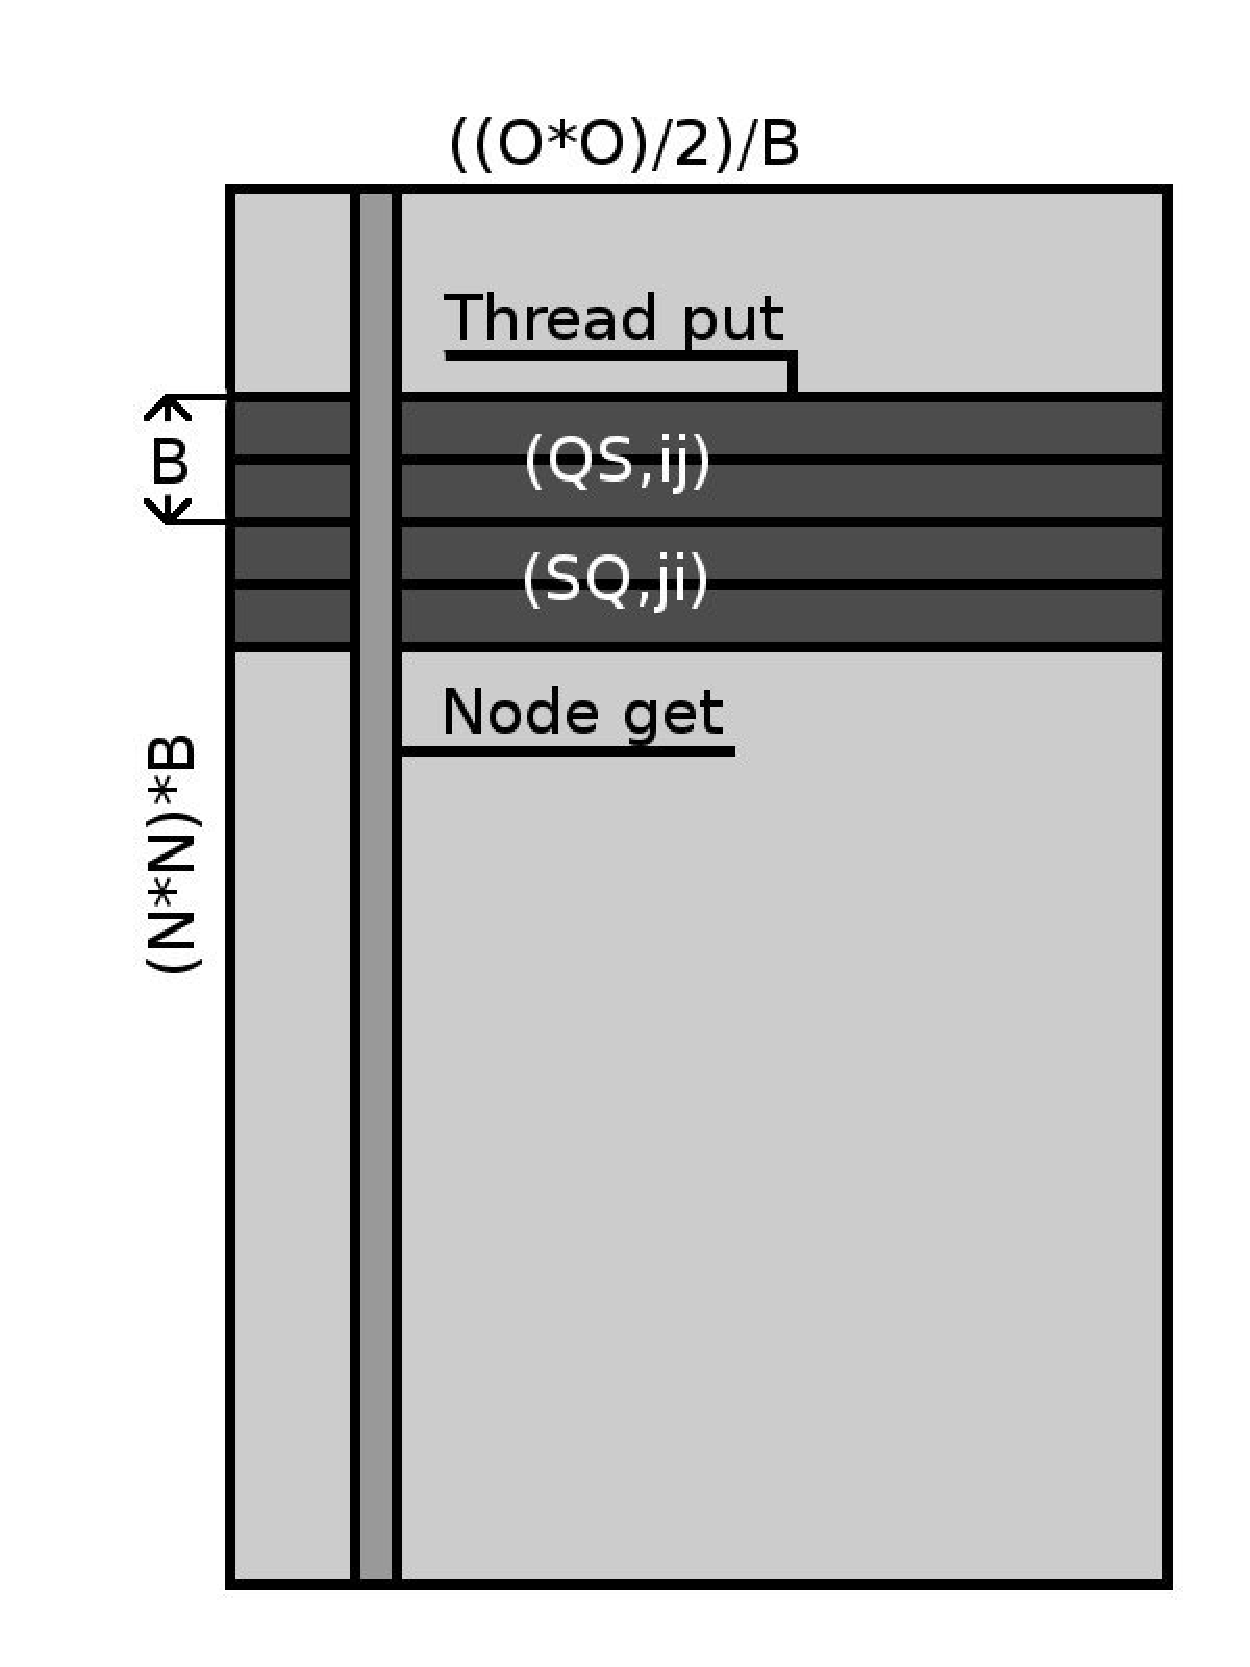
\includegraphics[scale=0.25]{figure.pdf}
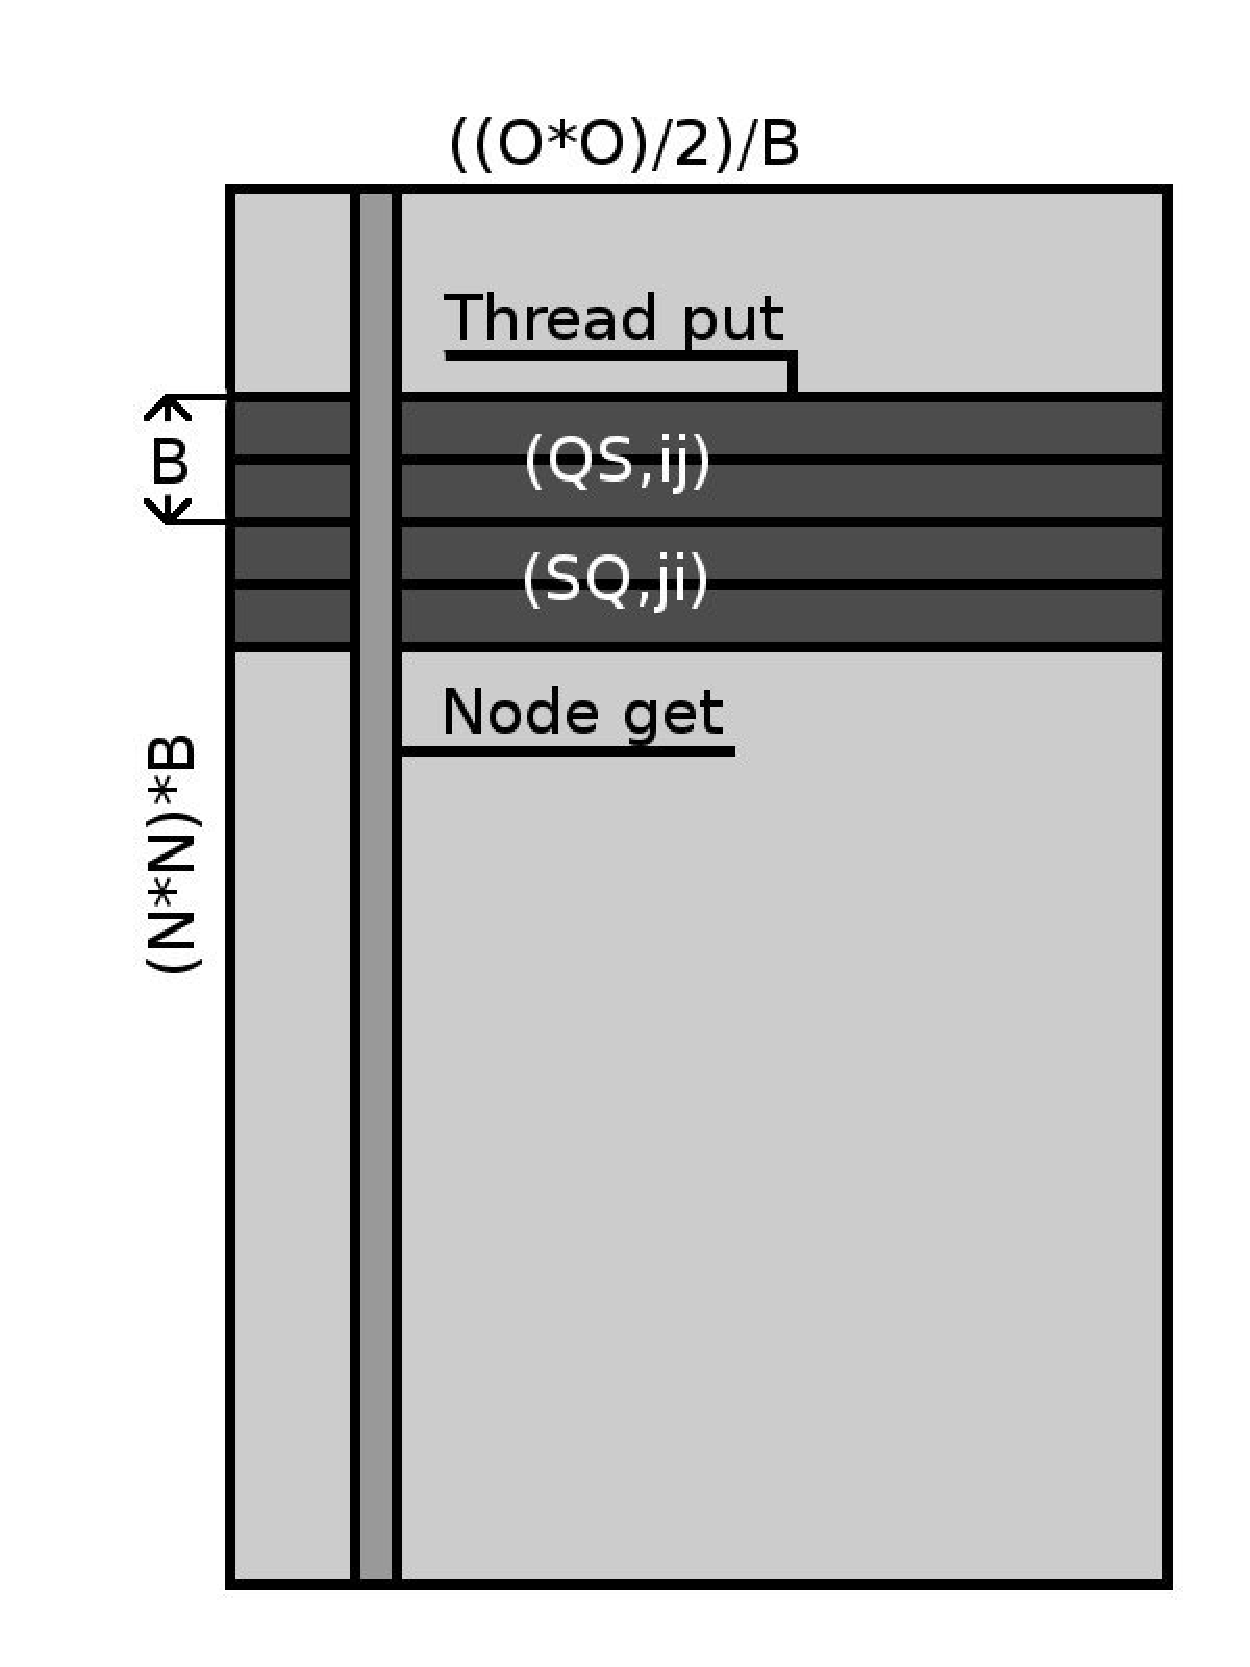
\includegraphics[scale=0.25]{figure.pdf}
\caption{Amplitude access patterns}
\label{patterns}
\end{center}
\end{figure}

Combining the above ideas, one can develop the following
algorithm, which has $(2*M^2*B,ij/B)$ and $(N^2B)$ I/O respectively,
Listing \ref{better}, with $M$ and $B$ factors determined by setting
runtime memory limits.

%\begin{lstlisting}[label=better, caption=Better approach, numbers=left]


\begin{listing}
\begin{verbatim}
B = ...; // some blocking factor, according to available memory
allocate V( N*N*B, (O^2/2)/B );
for (S,Q) in Blocks(Q <= S, M) {
  // block QS pairs into blocks of M functions 
  for R in Shells.blocks {
    for P in Shells.blocks {
      // skip insignificant ints
      eri.screen(P,Q,R,S));
      t_(i,S,R,Q) = eri(S,R,Q,P)*C(i,P);
      t1(i,S,Q,R) += t_(i,S,R,Q);
    }      
    t2(j,i,S,Q) = t1(i,S,Q,R)*C(j,R);
  }
  t(QSB,ij/B) = t2(j,i,S,Q); // the shell order is scrambled
  V(QSB,ij/B) = t(QSB,ij/B); // write block
  V(SQB,ji/B) = t(QSB,ij/B); // and symmetrical transpose
}
// 4/3 index
for ij in (O^2/2)/B {
  t(QSB) = V(QSB,ij);
  for (i,j) in B {
    t2(Q,S) = t(QS(i,j)); // unscramble shell order
    t3(a,S) = t2(Q,S)*C(a,Q)
    t4(a,b) = t3(a,S)*C(b,S);
    E += Energy(t4);
  }
}
\end{verbatim} \\
\hline
\caption{Better approach}
\label{better}
\end {listing}

%\end{lstlisting}


The main points about the above implementation:
\begin{itemize}
\item The amplitude symmetry is exploited in Q,S shells.  The
  half-transformed integrals are written independently and can
  be computed in parallel.
\item The QS list is processed in terms of blocks of shell pairs,
  rather than individual shells pairs.  The optimal block size will
  depend on the available memory.  The bigger the block size, the
  better in general.
\item The transformed integrals are scrambled such that shells are
  interleaved with blocks of $ij$ indices of size B.  The contiguous
  size of this noncontiguous write is $2*M^2*B$.
\item The 3rd/4th transformation reads the contiguous interleaved
  blocks.  The shell order is unscrambled one occupied pair at a time,
  the unscrambled block is transformed and the corresponding energy is
  computed.
\item The read operation to fetch next block can overlap with computation.  
\end{itemize}

The 2 innermost transformations are responsible for most of the
computational work, therefore it is important to have it as efficient
as possible in terms of performance and memory footprint.  For any any
given shell pair $(q,s)$, the $(P,R)$ list is evaluated in terms of
blocks off identical shells, to minimize integral initialization
overhead.  Each individual block is contracted to first occupied
index.  Once a given $R$ block is finished, it is then transformed to
second occupied index.  each transformation can be carried out using
{\tt dgemm}, making sure that screened out integrals are absent from
transformation.

\section{Performance}
There are a number of points which are useful to judge performance,
scalability, and flexibility of the algorithm:

\begin{itemize}
\item How the new approach compares to similar algorithm
\item how to network interface affects performance
\item The relative time spent in ERI, transforms, and I/O
\end{itemize}

First, lets compare performance to DDI and IMS implementations in
gamess to show poor performance of the former and excellent
performance of the latter on an average cluster connected by
InfiniBand.  The two inputs are a Taxol molecule, with small 6-31G and
larger 6-31Gd basis, Table \ref{small}.  The DDI code is extremely slow
compared to both, the IMS and the current implementation, by more than a
factor of 10X.  Furthermore, DDI MP2 memory requirement scales as $ON^2$
making it suitable only for small calculations: anything beyond 1000
atomic basis functions would require over 1GB of local memory per
core, leaving little room to scale.

\begin{table}
  \label{small}
  \caption {Small Benchmarks, compared to
    DDI \cite{fletcher1997parallel} and IMS \cite {ishimura2006new}.}
  \begin{center}
    \begin{tabular}{| l | c | c | c | c |}
      \hline
      Input        & Cores & DDI   & IMS  & New  \\ 
      \hline
      Taxol/6-31G  & 24    & 39.7  & 3.7  &  3.1  \\
      Taxol/6-31Gd & 36    & 86.3  & 7.5  &  5.4 \\
      \hline
    \end{tabular}
  \end{center}
\end{table}

The next set of benchmarks to illustrate advantage of the new
approach over the IMS algorithm are Taxol/cc-pVDZ and
19H20/aug-cc-pVTZ.  The Taxol/cc-pVDZ computation involves 1185 basis
functions, 164 occupied and 959 virtual orbitals.  The
19H20/aug-cc-pVTZ computation involves 1995 basis functions, 162
occupied and 1653 virtual orbitals.
The first input is less computation intensive but requires 50\%  more
storage and consequently I/O whereas the second input is
computation heavy due to diffuse (less screening) functions.

\begin{table}
  \label{medium}
  \caption {Small Benchmarks, compared to IMS \cite {ishimura2006new} }
  \begin{center}
    \begin{tabular}{| l | c | c | c | c | c |}
      \hline
      Input & 6 cores & IMS/6 cores & 60 cores/1GbE & 60 cores/IB & IMS/60 cores \\ 
      \hline
      Taxol & 76.0    & 116.6       & 19.3          & 7.9         & 10.7         \\
      19H20 & 458.3   & 858.5       & 50.5          & 45.7        & 95.0         \\
      \hline
    \end{tabular}
  \end{center}
\end{table}

The new implementation is a clear improvement over the existing IMS disk
algorithm, especially when diffuse functions
are present, being faster by almost factor of two.  The
implementation scales on small cluster, even when running over an
Ethernet interface, although more I/O bound Taxol calculation
performance deteriores quickly.  In case of computationally heavy
water cluster input, the difference between Ethernet and InfiniBand is
about 10\%.

The breakdown of each step of calculation is given in Table \ref
{breakdown}.  In both cases the integral calculation accounts for
significant fraction of time.  The water cluster calculation has
almost all of its work concentrated in the integral and first
transformation part due to much less screening, as opposed to sparser
Taxol calculation.  In both cases, the total I/O accounts for around
1\% of total runtime.  If the computational power were to suddenly
increase, the algorithm would still be viable.

\begin{table}
  \label{breakdown}
  \caption {calculation breakdown}
  \begin{center}
    \begin{tabular}{| l | c | c | c | c | c | c | c |}
      \hline
      Input & Eri   & T1    & T2   & WRITE & READ & T3+T4 & sync \\ 
      \hline
      Taxol & 38.2  & 28.9  & 6.2 & 0.77  & 0.37 & 23.7   & 1.9 \\
      19H20 & 39.3  & 45.5  & 6.1  & 0.003 & 0.7  & 4.0   & 4.4  \\
      \hline
    \end{tabular}
  \end{center}
\end{table}


The next set of benchmarks is to illustrate capability the algorithm
on a large cluster, Cray XE6.  Two inputs are used, Taxol/aug-cc-pVDZ
and Valinomycin/cc-PVTZ.  When considering timings given below, is
important to keep in mind that those numbers are for one thread only
and do not give the exact nature of the system as a whole.

The smaller Taxol computation has 164 active occupied, 1659 virtual,
and 2009 atomic orbitals, with 500GB integral storage.  The storage is
small enough to fit in distributed memory.  The computation times and
percentage by step is given in Table \ref {taxol}.  The run with
filesystem storage takes 17\% longer, which can be expected
considering the 64:1 compute to I/O ratio.  When running in
distributed memory entirely, the I/O overhead is hardly noticeable,
due to fast Gemini interconnect.  The super-linear speed-up is most
likely due to cache effects of reduced memory pressure on individual
nodes.

\begin{table}
  \label{taxol}
  \caption {Taxol/aug-cc-pVDZ}
  \begin{center}
    \begin{tabular}{| c | c | c | c | c | c | c | c | c |}
      \hline
      Cores & Time & Eri   & T1    & T2   & WRITE & READ & T3+T4 & sync \\ 
      \hline 
      512 & 63.9 & 14.1 & 52.8 & 10.0 & 0.1 & 3.5 & 5.5 & 14.0 \\
      512 & 52.5 & 17.2 & 53.1 & 15.4 & 0.1 & 0.1 & 8.1 & 6.0 \\
     1024 & 25.3 & 18.2 & 40.6 & 9.9  & 0.1 & 0.1 & 8.4 & 22.7 \\
      \hline
    \end{tabular}
  \end{center}
\end{table}


The larger computation, Valinomycin/cc-PVTZ, has 222 active occupied,
3300 virtual, and 4080 atomic orbitals.  The storage required for this
computation is 3.3TB requiring file storage.  The amplitude file is
stored on Lustre filesystem, 8 I/0 nodes, and stripping size set to
32MB.  The computation times and percentage by step is given in Table
\ref {valinomycin}.  For this computation the I/O overhead is
significant, on the order of 25\%, again due to more effective
screening in the absence of diffuse functions.  The scalability
suffers as well, both due to more I/O and unfavorable 64:1 compute to
I/o ratio when running on 512 cores.  Nevertheless, running the
calculation that would otherwise {\it require} around 2000 cores should
illustrate efficacy of the algorithm and flexible memory/filesystem
storage.

\begin{table}
  \label{valinomycin}
  \caption{Valinomycin/cc-pVTZ}
  \begin{center}
    \begin{tabular}{| c | c | c | c | c | c | c | c | c |}
      \hline
      Cores & Time & Eri   & T1    & T2   & WRITE & READ & T3+T4 & sync \\ 
      \hline
      256 & 313.8 & 17.8  & 16.4  & 18.0 & 9.3  & 17.5 & 18.2  & 2.8 \\
      512 & 204.6 & 7.2   & 20.5  & 16.3 & 18.1 & 7.1  & 28.3  & 2.5  \\
      \hline
    \end{tabular}
  \end{center}
\end{table}


\section{GPU Implementation}
There is a considerable interest in porting core quantum chemistry
algorithms to GPU.  Previously we were able to get moderate
performance with Hartree-Fock code \cite {asadchev}.  However, the MP2
GPU implementation turned out to be much less successful.

The following points about innermost implementation kernels must be
first highlighted:
\begin {itemize}
\item The integral block evaluated at once is relatively small, to
  keep the memory footprint low.
\item The integrals are screened, therefore the coefficient matrix
  needs to be repacked according to block-sparse structure of the
  integral block.
\item The first transformation is a series of relatively
  small matrix matrix multiplications.
\end {itemize}

While the CPU can handle the above tasks rather efficiently, the GPU
runtime is inefficient at handling many small tasks, rather than few
large tasks.  As a result, the GPU is poorly utilized, even if
using multiple streams to run several small kernels simultaneously.

The results of utilizing GPU using this particular approach a
disappointing: the average performance gain was less than 10\% over a
single CPU core.  Although the overall performance of the algorithm is
superior, especially over DDI algorithm, the main contribution is due
to better algorithm implementation itself rather than the raw
performance of the GPU.

The only place where GPU math libraries could make a difference are
the last two transformations where the bulk of work is handled by two
large consecutive matrix multiplies.  However they don't account for
much of the runtime, 30 \% at most in the above examples.  Speeding up
those alone computations is unlikely to improve general case
performance significantly. 

 The above finding does not mean an efficient MP2 GPU algorithm is not
 possible.  However, to achieve good GPU utilization, an approach
 significantly different from the above is needed.  This is in
 contrast from RI-MP2 GPU implementations \cite{watson2010accelerating} where the bulk of work is
 handled by few large matrix multiplies without the need to accomodate
the  integral sparcity directly.

\section{Conclusions}
The work described in this paper offers an improvement over the
existing MP2 energy algorithms both in terms of execution time and
resources utilization. A flexible data storage model allows to
transparently use either filesystem or distributed memory to store
partially transformed integrals.  A number of sample calculations
showed implementation to work well with small clusters and scale into
thousands of cores on Cray supercomputer.  However, translating the
CPU approach into GPU implementation proved to be unsuccessful, since
the GPU runtime handles the workload composed of large number of small
computations poorly.

\bibliographystyle{unsrt}% (uses file ``plain.bst'')
\bibliography{references}
\documentclass{beamer}
\usepackage[latin1]{inputenc}
\usetheme{Warsaw}
\title[ Software Design In Computational Sciences]{Software Design In Chemistry}
\author{ Andrey Asadchev}
\institute{Iowa State University}
\begin{document}

\begin{frame}
\titlepage
\end{frame}


\begin{frame}{Outline}
\begin{itemize}
\item Programming Languages
\item Object Oriented Programming
\item C++ and Python
\item Symbolic Computation
\item Current Computer Architectures
\item Computational Chemistry
\item Integral Evaluation
\item Fock Matrix
\item GPU Implementation
\item Performance
\item Conclusions
\end{itemize}
\end{frame}

\begin{frame}{Programming languages}
\begin{itemize}
\item Communicate To Computer And To Humans
\item Binary Machine Language - instructions as sequence of zero and one
\item Assembly - mnemonic shortcuts to machine language
\item Fortran - early imperative programming language.\\
  Numerical and matrix computations.
\item LISP - functional programming language.\\
   Stands for List Processor.\\
   Functions (as in mathematics) are first-class citizens.\\
   To Iterate Is Human, To Recurse Is Divine.\\
   Lambda functions and predicates: $G = map(lambda\, x,y: x*y, F,reversed(G))$\\
   Artificial Intelligence\\
\item C - Portable Assembly Language.\\
  developed together with UNIX operating system.\\
  System Programming Language.\\
  Access to the raw memory.
\end{itemize}
\end{frame}



\begin{frame}{ Object-Oriented Programming}
\begin{itemize}
\item Abstract implementation problem 
\item Keep Data and Methods together
\item Hide Data, Puts Constraints on Data
\item Polymorphism 
\item Inheritance
\item Matrix\\
Represented As Some Object M\\
M.transpose()\\
const M.m\\
Orthogonal Matrix Is a Matrix\\
Orthogonal Matrix Has Transpose\\
Orthogonal Matrix  has inverse\\
\end{itemize}
\end{frame}


\begin{frame}{  C++}
\begin{itemize}
\item Superset of C
\item Object Oriented
\item Functional
\item Widely Used, Many Compilers
\item Efficient, games programming and digital signal processing
\item Overload operators, + , *,...
\item Program formulas almost like on the paper\\
$Vector\, r = v-w $\\
\item Template meta-programming\\
 Generic Programs\\
 Automatically Generated Programs\\
 Specialized Programs\\
 Boost\\
Domain Specific Language And Template Expressions\\
Readability: $Quartet \langle Shell \rangle$
\end{itemize}
\end{frame}

\begin{frame}{  Python}
\begin{itemize}
\item Interactive,compiled 
\item Imperative
\item Object Oriented
\item Functional
\item Easy interfacing with other languages
\item Pythonic\\
 L = sorted([(x,y) for x in X for y in Y if x is y])
\item Widely Used in Science and Mathematics\\
pyQuante
\item  Template-preprocessor engines (PHP)\\
  Cheetah\\
Preprocessor directives directly embedded in program\\
\end{itemize}
\end{frame}

\begin{frame}{ Symbolic computations}
\begin{itemize}
\item Computed Expressions Without Explicitly Knowing Number
\item Computer Algebra Systems
\item Mathematica.\\
  Polynomial Manipulation\\
Matrix Manipulation\\
Recursion\\
Allows to Define Your Own Algebra\\
\item  Sage.\\
    Python Computer Algebra System\\
    Interface to almost any other computer algebra system
\item Sympy - symbolic python library.\\
\item  Put Equations As They Are.\\
Let Computer Algebra System Simplify Them\\
Use Program Generator to produce code as you  wanted\\
Optimize equations which otherwise would be prohibitive to
\end{itemize}
\end{frame}

\begin{frame}{ Computer Architecture}
\begin{itemize}
\item Pipeline
\item Single Instruction Multiple Data
\item Memory Locality
\item Many cores
\item Complex Scheduling
\item Very Hard to Beat a Compiler for Low-Level Optimization\\
however programs have to be written in such way as to be amenable to optimization\\
Conditional statements, unpredictable memory access prohibit optimization.
\item Processors Are Powerful and Cheap\\
     Optimized for Games and Signal Processing, 4x4 matrix\\
     Underutilized often, 15 percent efficiency is common
\item  Efficient Implementations demand unrolling kernels
\end{itemize}
\end{frame}

\begin{frame}{ Computer Architecture}
\begin{itemize}
\item 
\item   Graphical Units\\
 A Lot Of Performance And Even More Hype\\
 Memory Bound Often\\
 Single Instruction Multiple Thread\\
 Imagine mapping each loop iteration to threads\\
 for i  = threadID,N,numThreads:  X(i) = aY(i)
\end{itemize}
\end{frame}

\begin{frame}{  Computational Chemistry}
\begin{itemize}
\item Electron Integrals $(ab|cd)$\\
  Domain Specific\\
  Define rest of computations
\item Lots of Computations, Lots of Memory
\item Data Screening, Symmetry
\item  Linear Algebra, BLAS
\item Legacy Code
\item MPQC, libint
\end{itemize}
\end{frame}

\begin{frame}{   Integral  evaluation}
\begin{itemize}
\item $(ab|cd) = \sum C_i \sum C_j \sum C_k \sum C_l [ij|kl] $
\item $(ab|cd) = (ba|cd) = (cd|ab)...$
\item many different combinations and permutations
\item SP functions
\item high angular momentum versus high confection order\\
$(fsp | fsp)$
\item gaussian basis, $e ^{-r^2}$ separable in Cartesian coordinates
\item  Most Integral schemes use recursive nature of gaussian integration/differentiation
\item Numerical error - loss of significant figures, etc.\\
Recursion implies using a slightly incorrect value to compute next\\
Especially severe when two values are close in magnitude but different in sign (difference)
\end{itemize}
\end{frame}

\begin{frame}{   Integral  evaluation}
\begin{itemize}
\item 
\item OS integral scheme, auxiliary integrals. \\
Very general - applicable to almost any operator\\
R12 linear integrals\\
Memory Hungry
\item Rys quadrature\\
  Gaussian quadrature using Rys orthogonal polynomials\\
  $I = \sum_a Ix(a)Iy(a)Iz(a)$\\
  Compute Roots\\
  Compute two-dimensional x, y, z intermediate integrals\\
  Assemble final integral
\item Horizontal recurrence\\
$(pp | = q*(ps |  + (ds |$\\
Simplifies Contracted Integrals\\
High Numerical Error
\end{itemize}
\end{frame}

\begin{frame}{  Integral Implementation}
\begin{itemize}
\item C++ object-oriented library
\item Fortran And Gamess bindings
\item  Simple Interface:\\
Create quadrature object for given shell quartet\\
Call Object operator for a given center quartet
call object operator for a list of Center quartets

\item Two Internal Implementations:\\
  Fully Unrolled And Simplified kernels for smaller  integral, 
  which is likely to be contracted\\
  Partially Unrolled (bra only) general quadrature\\
\item Internals make heavy use of  C++ templates and automatically generated code
\item Human Serviceable Code is small - around 2000 lines of code
\item Final Library Size his small - around 5 megabytes fully optimized
\item the code is kept small due to objects and genetic templates
\end{itemize}
\end{frame}

\begin{frame}{  Fock Matrix}
\begin{itemize}
\item $F = (ab |cd)D $
\item Part of the Library
\item Requires Matrix to be in block form through an adapter
\item Simple Interface:\\
Create fock object for given shell quartet\\
Call Object operator for a given center quartet\\
Call Object operator for a list of Center quartets
\item Two Internal Implementations - parallel to those of integral program
\item Basis Set organization and higher-level logic is handled by another library
\end{itemize}
\end{frame}

\begin{frame}{  GPU implementation}
\begin{itemize}
\item Implementations are driven by integral size and contraction order
\item Large integrals are parallel over individual elements\\
every thread gets a unique internal element to compute
\item highly contracted small integrals are parallel over contractions\\
every thread gets the unique contraction to compute\\
contractions are  reduced in the end
\item Basis  must be ordered to guarantee execution of the kernel on multiple centers
\item Thanks to objects and genetic templates, the entire kernel code is about 300 lines
\end{itemize}
\end{frame}

\begin{frame}{   Performance}
\begin{itemize}
\item GPU implementation not yet complete
\item CPU implementation:\\
  benchmark several cases from hundred to a thousand basis functions\\
  largest test is loperamide 6-31G(pdf)
  numerical agreement to 8 decimal places\\
  30-40\% improvement in speed\\
  Fine grain contraction screening was not enabled\\
  Intel compiler generates vector instructions\\
  still working on full optimization
\item GPU implementation not yet complete\\
  basic integrals, up to the 1500 quartet size are working\\
  50\% improvement over CPU\\
  numbers essentially agree
\end{itemize}
\end{frame}


\begin{frame}{Aknowledge}
\begin{itemize}
\item Funding From Dr. Gordon
\item  Help From Jacob and Allada
\end{itemize}
\end{frame}

\end{document}


\end{document}



% LocalWords:  
